%%____________________________________________________________________________||
\section{Data sets}
\label{sec:datasets}

\subsection{Data}

In this note, we use proton-proton collision data at $\sqrt{s} =$ 13~TeV
being collected in 2015. Table~\ref{tab:datasets_data} lists the names of
the data sets relevant for the analysis. The integrated luminosities
shown in the table are the sizes of the certified data for each data set
at the time of writing. Since the data collection for the year 2015 and
the certification of the data are ongoing, the sizes of the data sets
that will be used in the final version of the note will be different
from the sizes that the table indicates.

This version of the note uses subsets of the data listed in the table.
As the analysis is actively ongoing, different sections of this note
might use different sizes of the data. The data sizes used in particular
studies in the note might be indicated in relevant sections, tables or
figures.

We are performing the blind analysis. In this version of the note, the
data in the signral region is blinded. In the signral region, only the
149.48 \ipb of the certified data agreed upton to unblind in the SUS PAG are
analysed. No data in the control regions is blinded.

\subsection{Simulation}

Table~\ref{tab:datasets_bkg} lists the data sets of simulated events
of the standard model background processes used in this note. In these
data sets, in addition to the main interaction, each event contains on
average 20 minimum bias interactions which simulate multiple
interactions per bunch-crossing (in-time pileup). The expected detector
signal from previous or following bunch crossings (out-of-time pileup)
with 25ns bunch spacing is overlapped.


\begin{table}[!h]
\topcaption{Data sets}
\footnotesize \begin{center}
\begin{tabular}{l}
\hline\hline
\multicolumn{1}{c}{Data set}\tabularnewline
\hline
\verb!/HTMHT/Run2016B-23Sep2016-v3/MINIAOD!\tabularnewline
\verb!/HTMHT/Run2016C-23Sep2016-v1/MINIAOD!\tabularnewline
\verb!/HTMHT/Run2016D-23Sep2016-v1/MINIAOD!\tabularnewline
\verb!/HTMHT/Run2016E-23Sep2016-v1/MINIAOD!\tabularnewline
\verb!/HTMHT/Run2016F-23Sep2016-v1/MINIAOD!\tabularnewline
\verb!/HTMHT/Run2016G-23Sep2016-v2/MINIAOD!\tabularnewline
\verb!/HTMHT/Run2016H-PromptReco-v2/MINIAOD!\tabularnewline
\verb!/HTMHT/Run2016H-PromptReco-v3/MINIAOD!\tabularnewline
\verb!/JetHT/Run2016B-23Sep2016-v2/MINIAOD!\tabularnewline
\verb!/JetHT/Run2016C-23Sep2016-v2/MINIAOD!\tabularnewline
\verb!/JetHT/Run2016D-23Sep2016-v2/MINIAOD!\tabularnewline
\verb!/JetHT/Run2016E-23Sep2016-v1/MINIAOD!\tabularnewline
\verb!/JetHT/Run2016F-23Sep2016-v1/MINIAOD!\tabularnewline
\verb!/JetHT/Run2016G-23Sep2016-v2/MINIAOD!\tabularnewline
\verb!/JetHT/Run2016H-PromptReco-v2/MINIAOD!\tabularnewline
\verb!/JetHT/Run2016H-PromptReco-v3/MINIAOD!\tabularnewline
\verb!/MET/Run2016B-23Sep2016-v3/MINIAOD!\tabularnewline
\verb!/MET/Run2016C-23Sep2016-v1/MINIAOD!\tabularnewline
\verb!/MET/Run2016D-23Sep2016-v1/MINIAOD!\tabularnewline
\verb!/MET/Run2016E-23Sep2016-v1/MINIAOD!\tabularnewline
\verb!/MET/Run2016F-23Sep2016-v1/MINIAOD!\tabularnewline
\verb!/MET/Run2016G-23Sep2016-v1/MINIAOD!\tabularnewline
\verb!/MET/Run2016H-PromptReco-v2/MINIAOD!\tabularnewline
\verb!/SingleMuon/Run2016B-23Sep2016-v3/MINIAOD!\tabularnewline
\verb!/SingleMuon/Run2016C-23Sep2016-v1/MINIAOD!\tabularnewline
\verb!/SingleMuon/Run2016D-23Sep2016-v1/MINIAOD!\tabularnewline
\verb!/SingleMuon/Run2016E-23Sep2016-v1/MINIAOD!\tabularnewline
\verb!/SingleMuon/Run2016F-23Sep2016-v1/MINIAOD!\tabularnewline
\verb!/SingleMuon/Run2016G-23Sep2016-v1/MINIAOD!\tabularnewline
\verb!/SingleMuon/Run2016H-PromptReco-v2/MINIAOD!\tabularnewline
\verb!/SingleMuon/Run2016H-PromptReco-v3/MINIAOD!\tabularnewline
\verb!/SinglePhoton/Run2016B-23Sep2016-v3/MINIAOD!\tabularnewline
\verb!/SinglePhoton/Run2016C-23Sep2016-v1/MINIAOD!\tabularnewline
\verb!/SinglePhoton/Run2016D-23Sep2016-v1/MINIAOD!\tabularnewline
\verb!/SinglePhoton/Run2016E-23Sep2016-v1/MINIAOD!\tabularnewline
\verb!/SinglePhoton/Run2016F-23Sep2016-v1/MINIAOD!\tabularnewline
\verb!/SinglePhoton/Run2016G-23Sep2016-v1/MINIAOD!\tabularnewline
\verb!/SinglePhoton/Run2016H-PromptReco-v2/MINIAOD!\tabularnewline
\verb!/SinglePhoton/Run2016H-PromptReco-v3/MINIAOD!\tabularnewline
\verb!/DoubleEG/Run2016B-23Sep2016-v3/MINIAOD!\tabularnewline
\verb!/DoubleEG/Run2016C-23Sep2016-v1/MINIAOD!\tabularnewline
\verb!/DoubleEG/Run2016D-23Sep2016-v1/MINIAOD!\tabularnewline
\verb!/DoubleEG/Run2016E-23Sep2016-v1/MINIAOD!\tabularnewline
\verb!/DoubleEG/Run2016F-23Sep2016-v1/MINIAOD!\tabularnewline
\verb!/DoubleEG/Run2016G-23Sep2016-v1/MINIAOD!\tabularnewline
\verb!/DoubleEG/Run2016H-PromptReco-v2/MINIAOD!\tabularnewline
\verb!/DoubleEG/Run2016H-PromptReco-v3/MINIAOD!\tabularnewline
\hline
\end{tabular}\end{center}

\label{tab:datasets_data}
\end{table}
\end{landscape}

\begin{landscape}
\begin{table}[!h]
\topcaption{Simulated background samples}
\tiny %latex.default(d, title = NULL, booktabs = FALSE, width = 3, rowname = NULL,     helvetica = FALSE, caption.loc = "bottom", ...)%
\begin{center}
\begin{tabular}{ll}
\hline\hline
\multicolumn{1}{c}{Data set}&\multicolumn{1}{c}{Cross section [pb]}\tabularnewline
\hline
\verb!/DYJetsToLL_M-10to50_TuneCUETP8M1_13TeV-amcatnloFXFX-pythia8/RunIISpring15DR74-Asympt25ns_MCRUN2_74_V9-v1/MINIAODSIM! &$1.861\times 10^{+04}$\tabularnewline
\verb!/DYJetsToLL_M-50_TuneCUETP8M1_13TeV-amcatnloFXFX-pythia8/RunIISpring15DR74-Asympt25ns_MCRUN2_74_V9-v3/MINIAODSIM! &$6.024\times 10^{+03}$\tabularnewline
\verb!/DYJetsToLL_M-50_HT-100to200_TuneCUETP8M1_13TeV-madgraphMLM-pythia8/RunIISpring15DR74-Asympt25ns_MCRUN2_74_V9-v2/MINIAODSIM! &$1.715\times 10^{+02}$\tabularnewline
\verb!/DYJetsToLL_M-50_HT-200to400_TuneCUETP8M1_13TeV-madgraphMLM-pythia8/RunIISpring15DR74-Asympt25ns_MCRUN2_74_V9-v2/MINIAODSIM! &$5.258\times 10^{+01}$\tabularnewline
\verb!/DYJetsToLL_M-50_HT-400to600_TuneCUETP8M1_13TeV-madgraphMLM-pythia8/RunIISpring15DR74-Asympt25ns_MCRUN2_74_V9-v2/MINIAODSIM! &$6.761\times 10^{+00}$\tabularnewline
\verb!/DYJetsToLL_M-50_HT-600toInf_TuneCUETP8M1_13TeV-madgraphMLM-pythia8/RunIISpring15DR74-Asympt25ns_MCRUN2_74_V9-v2/MINIAODSIM! &$2.718\times 10^{+00}$\tabularnewline
\verb!/GJets_HT-40To100_TuneCUETP8M1_13TeV-madgraphMLM-pythia8/RunIISpring15DR74-Asympt25ns_MCRUN2_74_V9-v2/MINIAODSIM! &$2.308\times 10^{+04}$\tabularnewline
\verb!/GJets_HT-100To200_TuneCUETP8M1_13TeV-madgraphMLM-pythia8/RunIISpring15DR74-Asympt25ns_MCRUN2_74_V9-v2/MINIAODSIM! &$9.110\times 10^{+03}$\tabularnewline
\verb!/GJets_HT-200To400_TuneCUETP8M1_13TeV-madgraphMLM-pythia8/RunIISpring15DR74-Asympt25ns_MCRUN2_74_V9-v2/MINIAODSIM! &$2.298\times 10^{+03}$\tabularnewline
\verb!/GJets_HT-400To600_TuneCUETP8M1_13TeV-madgraphMLM-pythia8/RunIISpring15DR74-Asympt25ns_MCRUN2_74_V9-v1/MINIAODSIM! &$2.730\times 10^{+02}$\tabularnewline
\verb!/GJets_HT-600ToInf_TuneCUETP8M1_13TeV-madgraphMLM-pythia8/RunIISpring15DR74-Asympt25ns_MCRUN2_74_V9-v1/MINIAODSIM! &$9.450\times 10^{+01}$\tabularnewline
\verb!/QCD_HT100to200_TuneCUETP8M1_13TeV-madgraphMLM-pythia8/RunIISpring15DR74-Asympt25ns_MCRUN2_74_V9-v2/MINIAODSIM! &$2.754\times 10^{+07}$\tabularnewline
\verb!/QCD_HT200to300_TuneCUETP8M1_13TeV-madgraphMLM-pythia8/RunIISpring15DR74-Asympt25ns_MCRUN2_74_V9-v2/MINIAODSIM! &$1.735\times 10^{+06}$\tabularnewline
\verb!/QCD_HT300to500_TuneCUETP8M1_13TeV-madgraphMLM-pythia8/RunIISpring15DR74-Asympt25ns_MCRUN2_74_V9-v2/MINIAODSIM! &$3.670\times 10^{+05}$\tabularnewline
\verb!/QCD_HT500to700_TuneCUETP8M1_13TeV-madgraphMLM-pythia8/RunIISpring15DR74-Asympt25ns_MCRUN2_74_V9-v1/MINIAODSIM! &$2.940\times 10^{+04}$\tabularnewline
\verb!/QCD_HT700to1000_TuneCUETP8M1_13TeV-madgraphMLM-pythia8/RunIISpring15DR74-Asympt25ns_MCRUN2_74_V9-v1/MINIAODSIM! &$6.524\times 10^{+03}$\tabularnewline
\verb!/QCD_HT1000to1500_TuneCUETP8M1_13TeV-madgraphMLM-pythia8/RunIISpring15DR74-Asympt25ns_MCRUN2_74_V9-v2/MINIAODSIM! &$1.064\times 10^{+03}$\tabularnewline
\verb!/QCD_HT1500to2000_TuneCUETP8M1_13TeV-madgraphMLM-pythia8/RunIISpring15DR74-Asympt25ns_MCRUN2_74_V9-v1/MINIAODSIM! &$1.215\times 10^{+02}$\tabularnewline
\verb!/QCD_HT2000toInf_TuneCUETP8M1_13TeV-madgraphMLM-pythia8/RunIISpring15DR74-Asympt25ns_MCRUN2_74_V9-v1/MINIAODSIM! &$2.542\times 10^{+01}$\tabularnewline
\verb!/QCD_Pt_80to120_TuneCUETP8M1_13TeV_pythia8/RunIISpring15DR74-Asympt25ns_MCRUN2_74_V9-v1/MINIAODSIM! &$2.763\times 10^{+06}$\tabularnewline
\verb!/QCD_Pt_120to170_TuneCUETP8M1_13TeV_pythia8/RunIISpring15DR74-Asympt25ns_MCRUN2_74_V9-v1/MINIAODSIM! &$4.711\times 10^{+05}$\tabularnewline
\verb!/QCD_Pt_170to300_TuneCUETP8M1_13TeV_pythia8/RunIISpring15DR74-Asympt25ns_MCRUN2_74_V9-v2/MINIAODSIM! &$1.173\times 10^{+05}$\tabularnewline
\verb!/QCD_Pt_300to470_TuneCUETP8M1_13TeV_pythia8/RunIISpring15DR74-Asympt25ns_MCRUN2_74_V9-v1/MINIAODSIM! &$7.823\times 10^{+03}$\tabularnewline
\verb!/QCD_Pt_470to600_TuneCUETP8M1_13TeV_pythia8/RunIISpring15DR74-Asympt25ns_MCRUN2_74_V9-v2/MINIAODSIM! &$6.482\times 10^{+02}$\tabularnewline
\verb!/QCD_Pt_600to800_TuneCUETP8M1_13TeV_pythia8/RunIISpring15DR74-Asympt25ns_MCRUN2_74_V9-v2/MINIAODSIM! &$1.869\times 10^{+02}$\tabularnewline
\verb!/QCD_Pt_800to1000_TuneCUETP8M1_13TeV_pythia8/RunIISpring15DR74-Asympt25ns_MCRUN2_74_V9-v2/MINIAODSIM! &$3.229\times 10^{+01}$\tabularnewline
\verb!/QCD_Pt_1000to1400_TuneCUETP8M1_13TeV_pythia8/RunIISpring15DR74-Asympt25ns_MCRUN2_74_V9-v1/MINIAODSIM! &$9.418\times 10^{+00}$\tabularnewline
\verb!/QCD_Pt_1400to1800_TuneCUETP8M1_13TeV_pythia8/RunIISpring15DR74-Asympt25ns_MCRUN2_74_V9-v1/MINIAODSIM! &$8.427\times 10^{-01}$\tabularnewline
\verb!/QCD_Pt_1800to2400_TuneCUETP8M1_13TeV_pythia8/RunIISpring15DR74-Asympt25ns_MCRUN2_74_V9-v1/MINIAODSIM! &$1.149\times 10^{-01}$\tabularnewline
\verb!/QCD_Pt_2400to3200_TuneCUETP8M1_13TeV_pythia8/RunIISpring15DR74-Asympt25ns_MCRUN2_74_V9-v1/MINIAODSIM! &$6.830\times 10^{-03}$\tabularnewline
\verb!/QCD_Pt_3200toInf_TuneCUETP8M1_13TeV_pythia8/RunIISpring15DR74-Asympt25ns_MCRUN2_74_V9-v1/MINIAODSIM! &$1.654\times 10^{-04}$\tabularnewline
\verb!/ST_tW_antitop_5f_inclusiveDecays_13TeV-powheg-pythia8_TuneCUETP8M1/RunIISpring15DR74-Asympt25ns_MCRUN2_74_V9-v1/MINIAODSIM! &$3.560\times 10^{+01}$\tabularnewline
\verb!/TTJets_TuneCUETP8M1_13TeV-amcatnloFXFX-pythia8/RunIISpring15DR74-Asympt25ns_MCRUN2_74_V9-v1/MINIAODSIM! &$8.318\times 10^{+02}$\tabularnewline
\verb!/TTJets_TuneCUETP8M1_13TeV-madgraphMLM-pythia8/RunIISpring15DR74-Asympt25ns_MCRUN2_74_V9-v2/MINIAODSIM! &$8.318\times 10^{+02}$\tabularnewline
\verb!/ST_s-channel_4f_leptonDecays_13TeV-amcatnlo-pythia8_TuneCUETP8M1/RunIISpring15DR74-Asympt25ns_MCRUN2_74_V9-v1/MINIAODSIM! &$3.681\times 10^{+00}$\tabularnewline
\verb!/ST_t-channel_4f_leptonDecays_13TeV-amcatnlo-pythia8_TuneCUETP8M1/RunIISpring15DR74-Asympt25ns_MCRUN2_74_V9-v1/MINIAODSIM! &$7.031\times 10^{+01}$\tabularnewline
\verb!/ST_tW_top_5f_inclusiveDecays_13TeV-powheg-pythia8_TuneCUETP8M1/RunIISpring15DR74-Asympt25ns_MCRUN2_74_V9-v1/MINIAODSIM! &$3.560\times 10^{+01}$\tabularnewline
\verb!/WJetsToLNu_TuneCUETP8M1_13TeV-amcatnloFXFX-pythia8/RunIISpring15DR74-Asympt25ns_MCRUN2_74_V9-v1/MINIAODSIM! &$6.153\times 10^{+04}$\tabularnewline
\verb!/WJetsToLNu_HT-100To200_TuneCUETP8M1_13TeV-madgraphMLM-pythia8/RunIISpring15DR74-Asympt25ns_MCRUN2_74_V9-v1/MINIAODSIM! &$1.630\times 10^{+03}$\tabularnewline
\verb!/WJetsToLNu_HT-200To400_TuneCUETP8M1_13TeV-madgraphMLM-pythia8/RunIISpring15DR74-Asympt25ns_MCRUN2_74_V9-v1/MINIAODSIM! &$4.356\times 10^{+02}$\tabularnewline
\verb!/WJetsToLNu_HT-400To600_TuneCUETP8M1_13TeV-madgraphMLM-pythia8/RunIISpring15DR74-Asympt25ns_MCRUN2_74_V9-v3/MINIAODSIM! &$5.917\times 10^{+01}$\tabularnewline
\verb!/WJetsToLNu_HT-600To800_TuneCUETP8M1_13TeV-madgraphMLM-pythia8/RunIISpring15DR74-Asympt25ns_MCRUN2_74_V9-v2/MINIAODSIM! &$1.549\times 10^{+01}$\tabularnewline
\verb!/WJetsToLNu_HT-800To1200_TuneCUETP8M1_13TeV-madgraphMLM-pythia8/RunIISpring15DR74-Asympt25ns_MCRUN2_74_V9-v1/MINIAODSIM! &$6.365\times 10^{+00}$\tabularnewline
\verb!/WJetsToLNu_HT-1200To2500_TuneCUETP8M1_13TeV-madgraphMLM-pythia8/RunIISpring15DR74-Asympt25ns_MCRUN2_74_V9-v1/MINIAODSIM! &$1.609\times 10^{+00}$\tabularnewline
\verb!/WJetsToLNu_HT-2500ToInf_TuneCUETP8M1_13TeV-madgraphMLM-pythia8/RunIISpring15DR74-Asympt25ns_MCRUN2_74_V9-v2/MINIAODSIM! &$3.738\times 10^{-02}$\tabularnewline
\verb!/WWTo2L2Nu_13TeV-powheg/RunIISpring15DR74-Asympt25ns_MCRUN2_74_V9-v1/MINIAODSIM! &$1.246\times 10^{+01}$\tabularnewline
\verb!/WZ_TuneCUETP8M1_13TeV-pythia8/RunIISpring15DR74-Asympt25ns_MCRUN2_74_V9-v1/MINIAODSIM! &$6.610\times 10^{+01}$\tabularnewline
\verb!/ZJetsToNuNu_HT-100To200_13TeV-madgraph/RunIISpring15DR74-Asympt25ns_MCRUN2_74_V9-v1/MINIAODSIM! &$3.450\times 10^{+02}$\tabularnewline
\verb!/ZJetsToNuNu_HT-200To400_13TeV-madgraph/RunIISpring15DR74-Asympt25ns_MCRUN2_74_V9-v1/MINIAODSIM! &$9.638\times 10^{+01}$\tabularnewline
\verb!/ZJetsToNuNu_HT-400To600_13TeV-madgraph/RunIISpring15DR74-Asympt25ns_MCRUN2_74_V9-v1/MINIAODSIM! &$1.346\times 10^{+01}$\tabularnewline
\verb!/ZJetsToNuNu_HT-600ToInf_13TeV-madgraph/RunIISpring15DR74-Asympt25ns_MCRUN2_74_V9-v1/MINIAODSIM! &$5.170\times 10^{+00}$\tabularnewline
\verb!/ZZ_TuneCUETP8M1_13TeV-pythia8/RunIISpring15DR74-Asympt25ns_MCRUN2_74_V9-v3/MINIAODSIM! &$3.180\times 10^{+01}$\tabularnewline
\hline
\end{tabular}\end{center}

\label{tab:datasets_bkg}
\end{table}
\end{landscape}

\subsection{Pileup reweighting}


The distribution of the numbers of the pileup interactions in the
simulated events is different from that in the data; the simulated
events contain, on average, a larger number of pileup interactions than
the data. We reweight simulated events to correct for this difference.
This procedure is called \textit{pileup reweighting}.

In analyses in CMS, the pileup reweighting is, in general, done in the
method recommended by the physics validation group
\cite{twiki-PdmVPileUpDescription}. However, since, at the time of
writing, the recommended method for the 2015 data is not available, we
use reweighting factors that we privately derive. We will use the
recommended method in later versions of the note.

The reweighting factors used in this version of the note is a function
of the number of the reconstructed vertices derived by comparing the
data and simulated events. The events which pass the trigger path
\verb!HLT_ZeroBias! is used in the derivation. The condition of this
trigger path is a bunch crossing. Therefore, the events virtually
contain only pilup interactions. For the simulated event sample, we use
the so-called the neutrino guns, listed in
Table~\ref{tab:datasets_neutrinoguns}. This sample also virtually
contain only pilup interactions. In contrast, the events in the signal
and control regions each has, in addition to the pilup interactions, the
main interaction that produces high-\PT jets, muons, electrons, photons,
or missing transverse momentum as described in
Section~\ref{sec:selection}.


\begin{table}[!h]
\topcaption{Simulated sample used in deriving pileup reweighting factors}
\footnotesize %latex.default(d, title = NULL, booktabs = FALSE, width = 3, rowname = NULL,     helvetica = FALSE, caption.loc = "bottom", ...)%
\begin{center}
\begin{tabular}{ll}
\hline\hline
\multicolumn{1}{c}{Data set}\tabularnewline
\hline
\verb!/SingleNeutrino/RunIISpring15DR74-Asympt25nsRaw_MCRUN2_74_V9-v2/MINIAODSIM! \tabularnewline
\hline
\end{tabular}\end{center}

\label{tab:datasets_neutrinoguns}
\end{table}

\begin{figure}[!b]
\centering
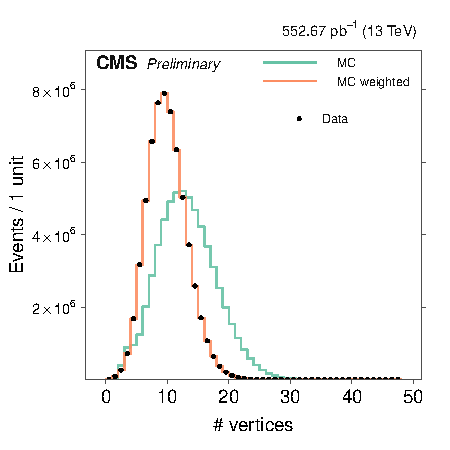
\includegraphics[scale=1.00]{figures/pileup_reweighting/f042_corr_nVert_data_mc_norm}
\caption{The distributions of the number of the reconstructed vertices
in the data, the simulated events, and the reweighted simulated events.
One is added to the the number of the reconstructed vertices.}
\label{f042_corr_nVert_data_mc_norm}
\end{figure}

The reweighting factors are derived as follows. First, we create the
distributions of the numbers of the reconstructed vertices for the data
and simulated sample. In creating these distributions, we add one to the
number of the reconstructed vertices. This is because these events do
not have the vetex for the main interaction while the events in the
signal and control regions do. Second, we smooth each distribution with
the smoothing spline. Third, we take the ratio of the two distributions,
i.e., the data over the simulated sample. The ratio is a function of the
number of reconstructed vertices. The ratio becomes reweighting factors
after normalised. The reweighting factors are normalised so as to
preserve the number of the generated events.

Figure~\ref{f042_corr_nVert_data_mc_norm} shows the distributions of the
number of the reconstructed vertices in the data, the simulated events,
and the reweighted simulated events. In the figure, one is added to the
the number of the reconstructed vertices. The figure demonstrates that
the reweighted simulated events have the distribution of the number of
the reconstructed vertices nearly identical to that in the data.


\subsection{Cross sections for SM samples}
Several MC samples of individual SM processes are binned according to a generator level quantity, such as the partonic \HT or bosonic \PT.
This analysis choses to use samples binned in partonic \HT, for the set of MC samples (W+jets, DY+jets, QCD, $\gamma$+jets, $Z\rightarrow \nu\nu$+jets) and $\hat{P_{T}}$
for only the QCD sample.
These binned samples are provided with LO cross sections. The \kfactors required to go from LO to NNLO cross setions are typically deterimned using corresponding
inclusive samples applied to each \HT binned sample.
Further studies can provide additional corrections to the cross sections, which can prove important to the closure test procedures described in
Section \ref{sec:closure-tests-desc}. As can be seen in Section \ref{sec:sideband_corrections}, residual cross section
corrections are measured using sidebands in data enriched specific processes.

Following an inclusive selection, the distribution of the MC samples with respect to the binning variable $H_{T}^{parton}$ are shown in Figure~\ref{fig:Lhe_Ht}, with
also the $\hat{P_{T}}$ distribution for QCD.

As stated above, the distributions shown in Figure~\ref{fig:Lhe_Ht} follow an inclusive selection, whereby there is no requirement on each event. This direct translation
from MC allows to fully stitch the binned generator level variable, and upon inspection appears to show a undeviating shape with respect to the cross section in question.

A more in depth, data-driven investigation into the cross sections is shown in Section \ref{sec:sideband_corrections}. Of which, an important point to note is that
the corrections to the cross sections, derived with the data sidebands are only relevant for data/MC comparison plots and the suite of closure tests defined in Section \ref{sec:closure-tests-desc}.

\begin{figure}[!h]
  \begin{center}
    \subfigure[$Z\rightarrow \nu\nu$ +jets] {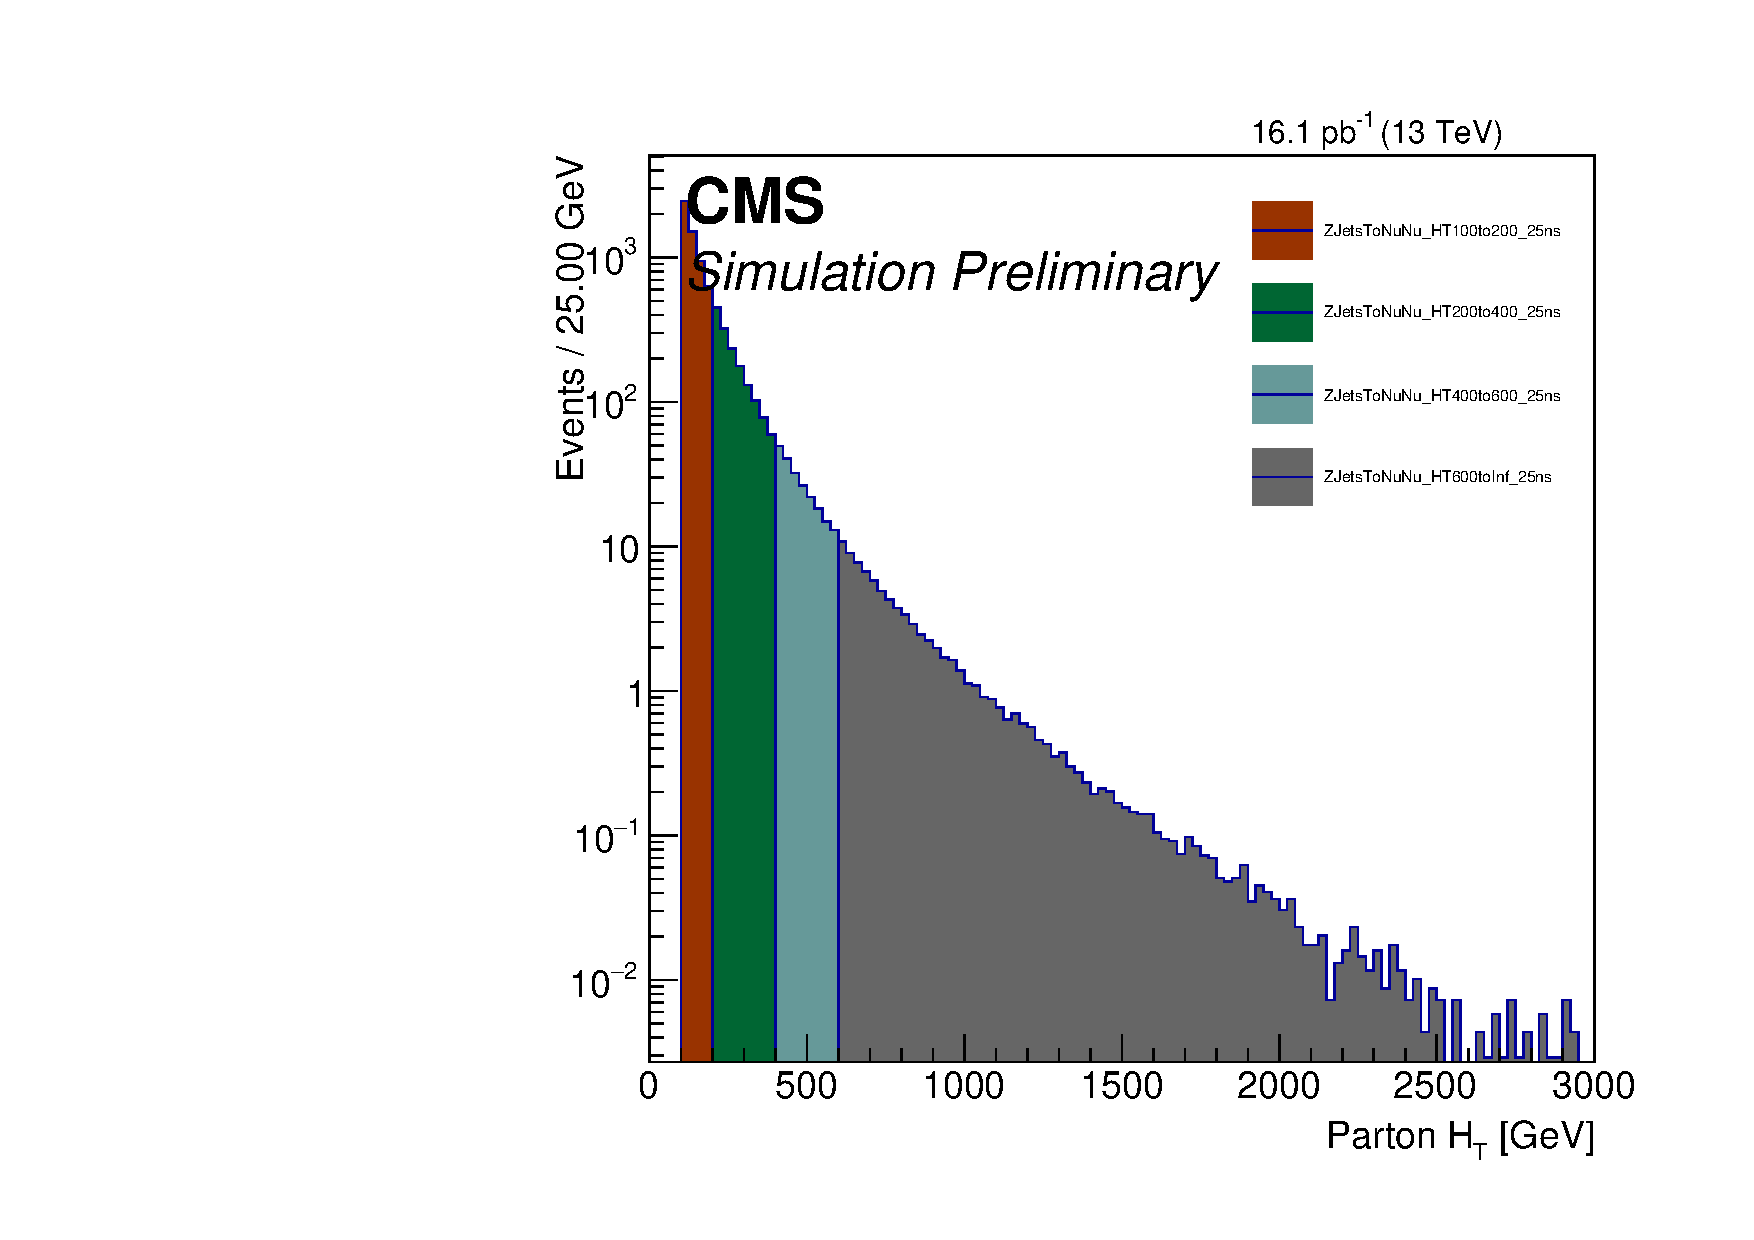
\includegraphics[width=0.45\textwidth]{figures/binnedMCsamples/Zinv.pdf}} ~~
    \subfigure[$W\rightarrow l \nu$ + jets]{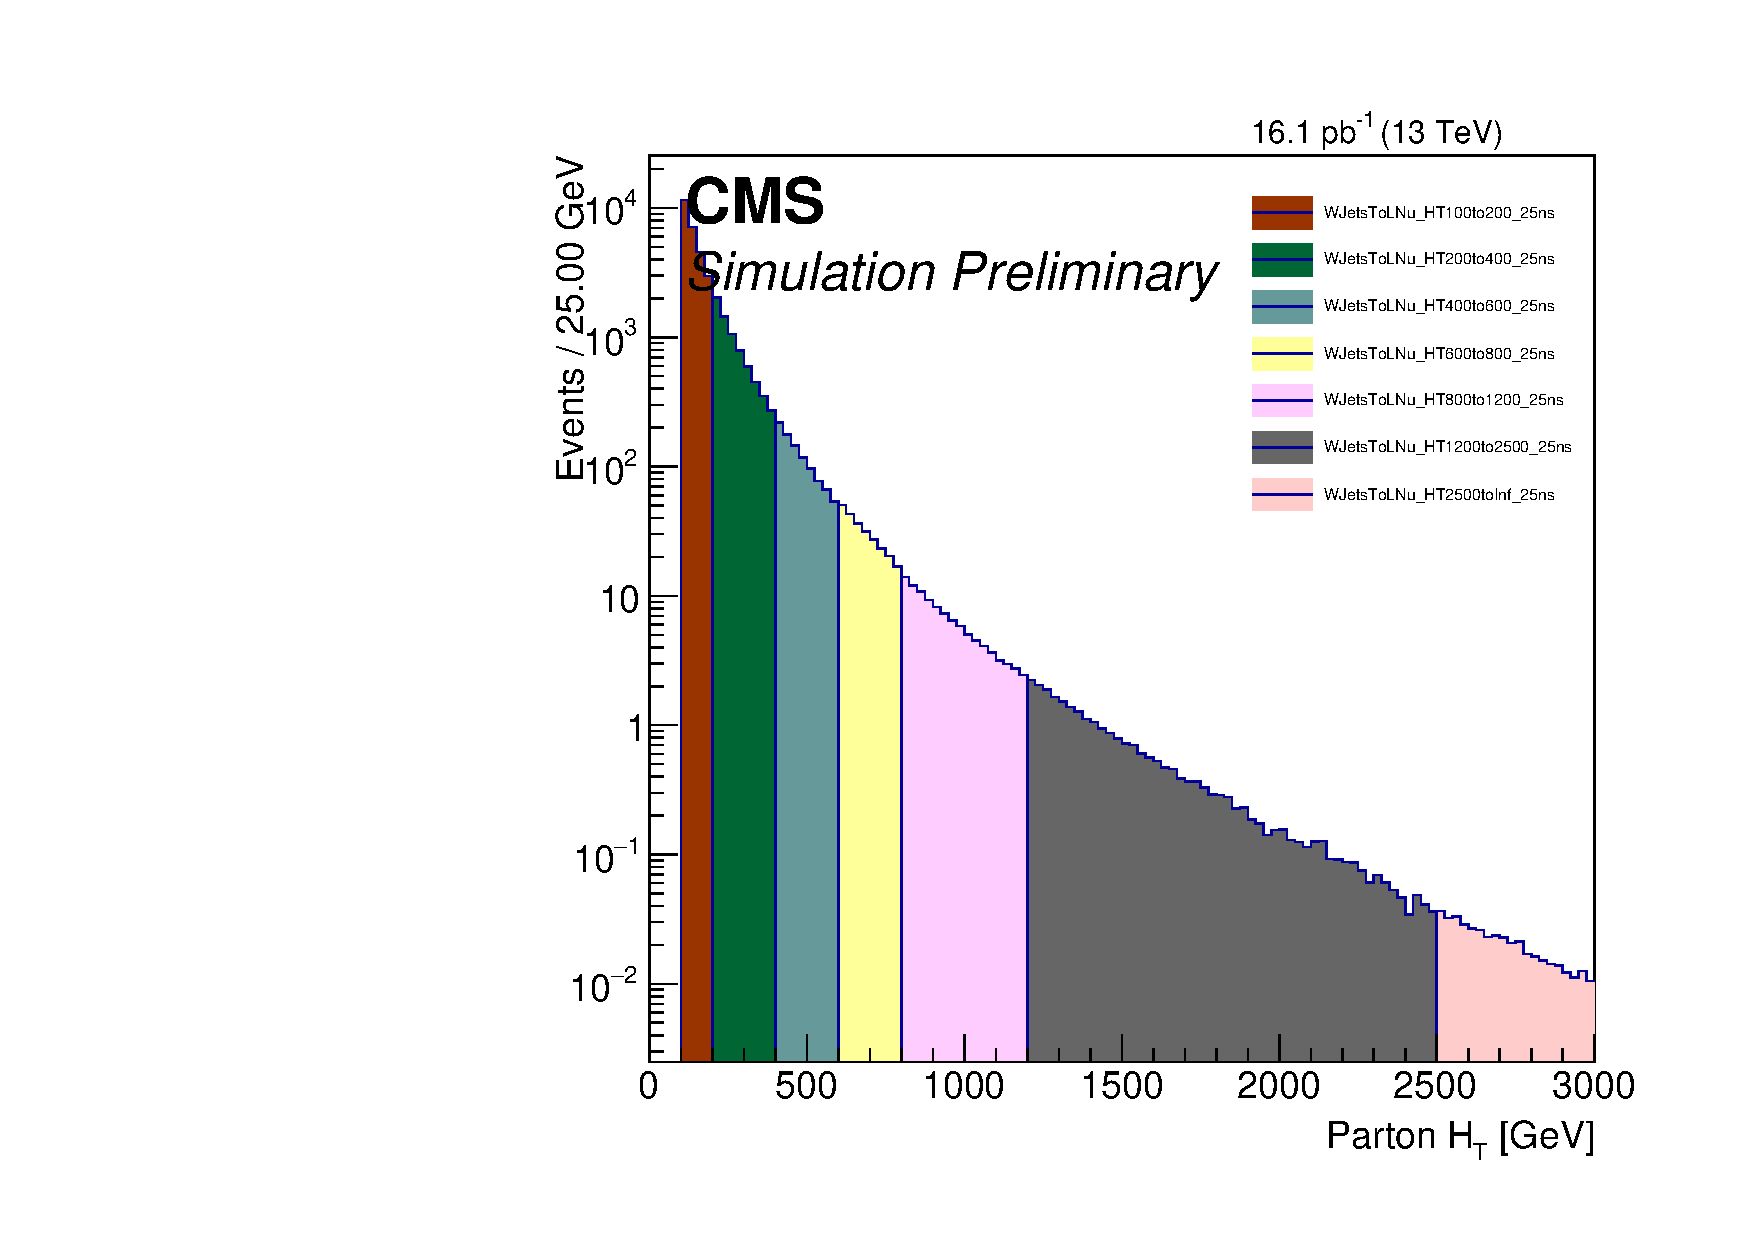
\includegraphics[width=0.45\textwidth]{figures/binnedMCsamples/WJetsToLNu_HT.pdf}} \\
    \subfigure[$DY\rightarrow ll$ + jets]{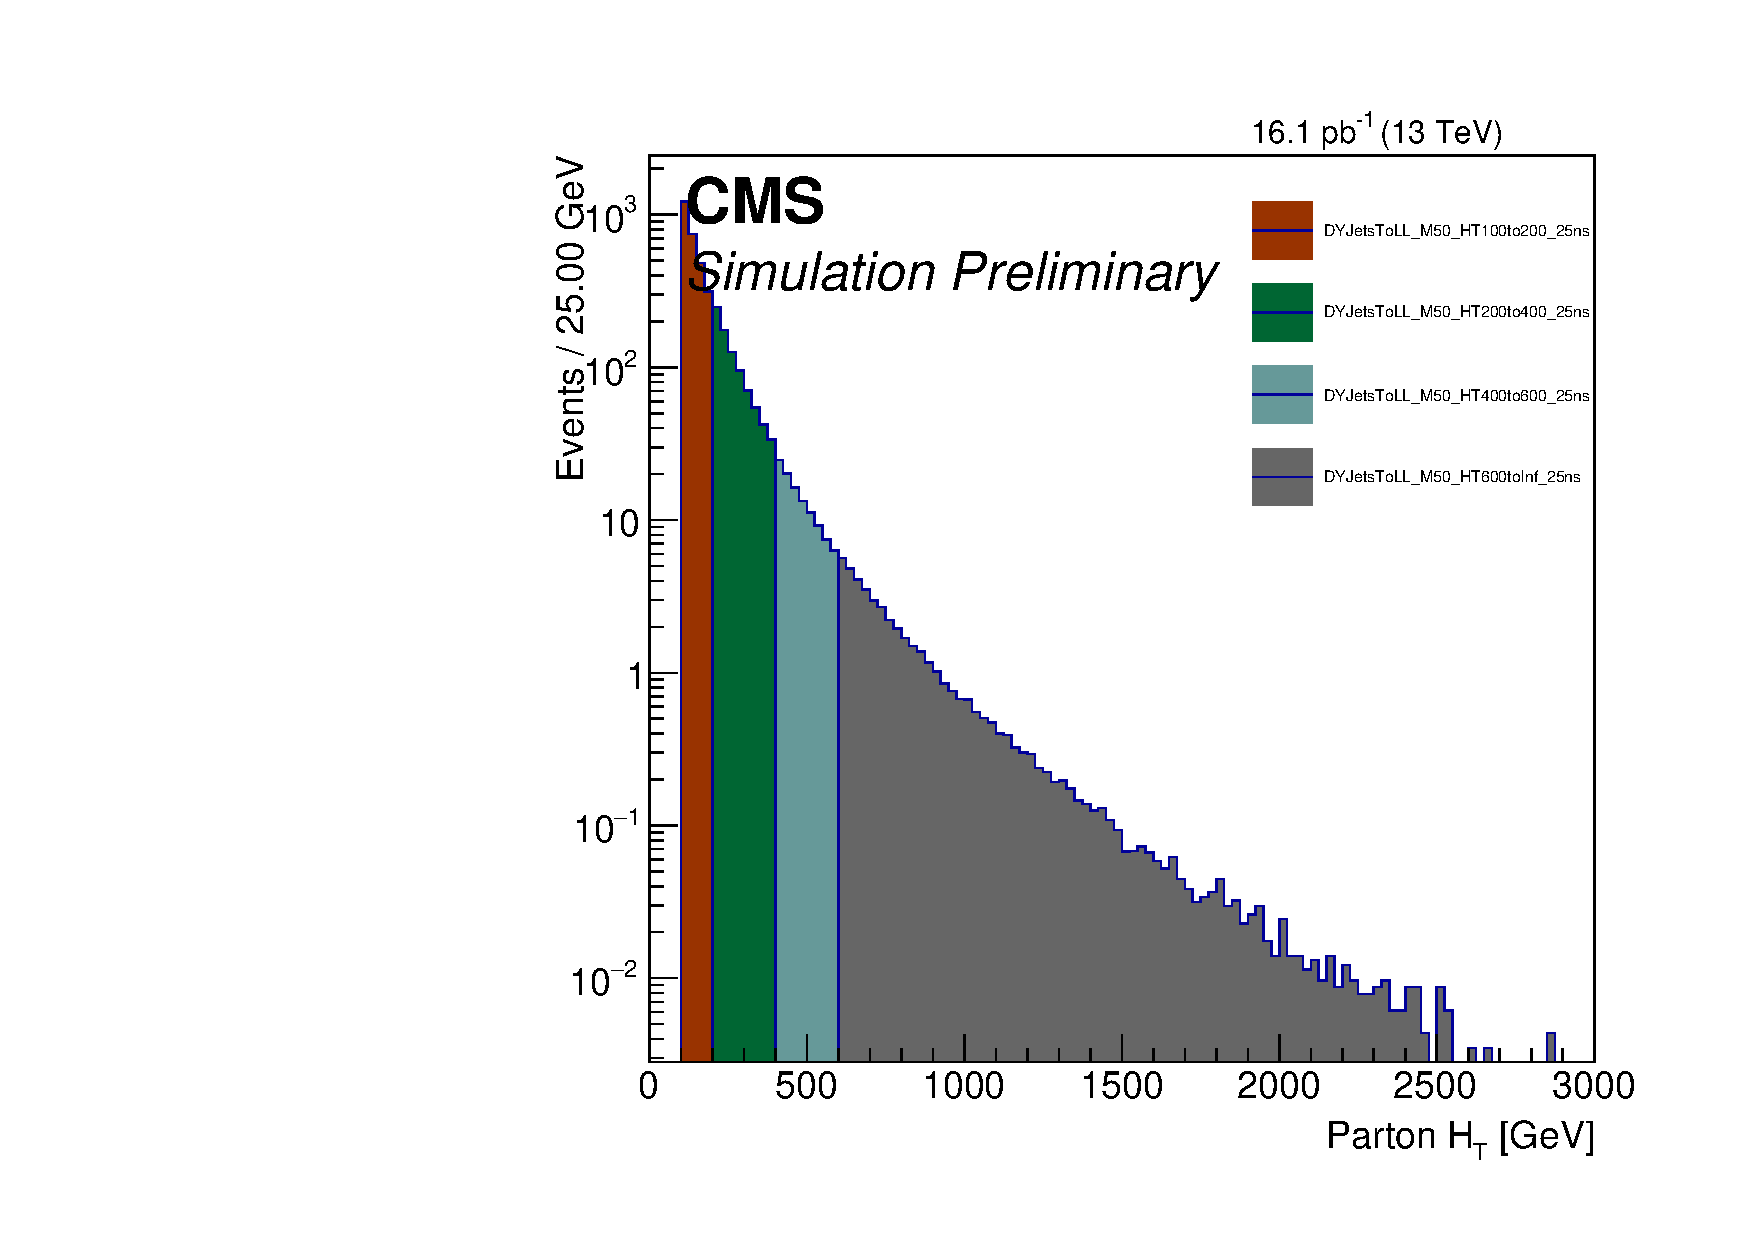
\includegraphics[width=0.45\textwidth]{figures/binnedMCsamples/DYJetsToLL_M50_HT.pdf}} ~~
    \subfigure[QCD]{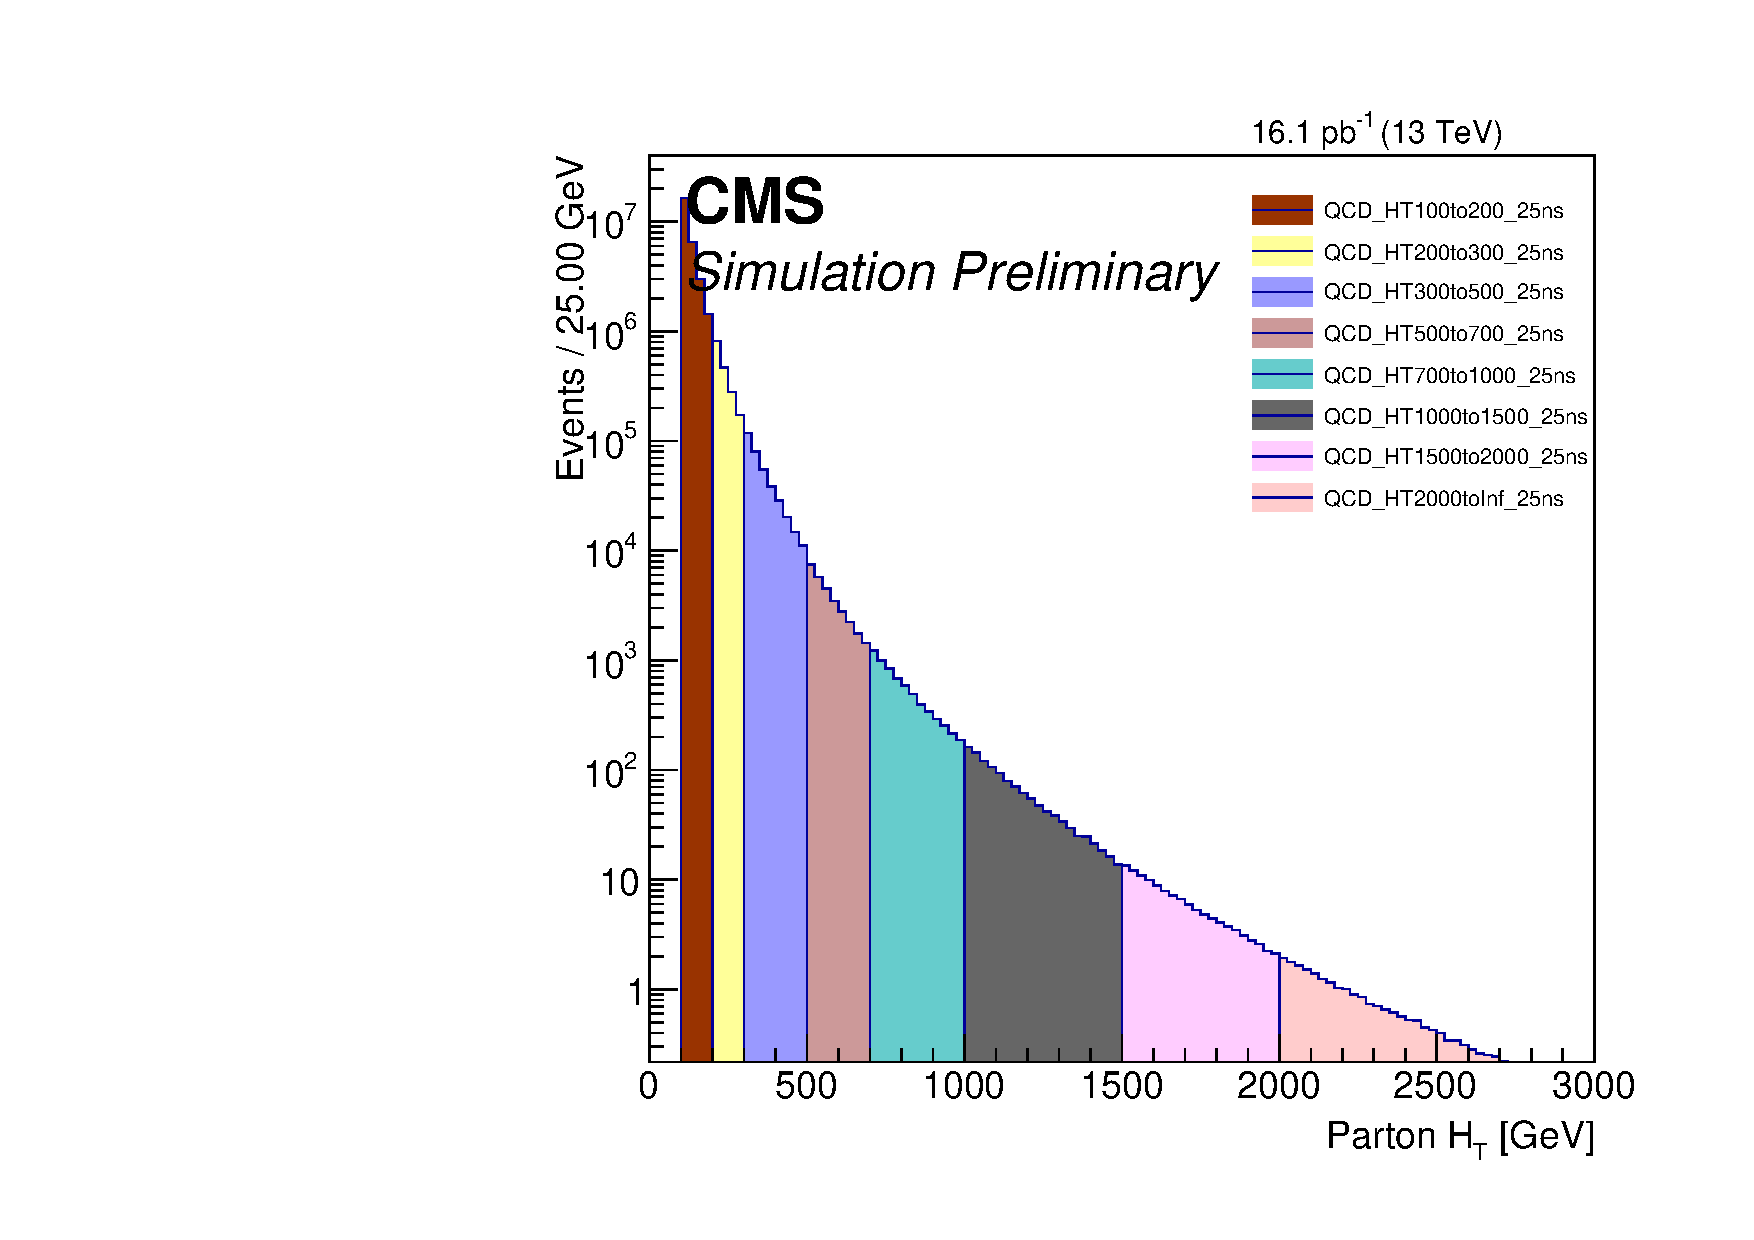
\includegraphics[width=0.45\textwidth]{figures/binnedMCsamples/QCD_HT.pdf}} \\
    \subfigure[$\gamma$+jets]{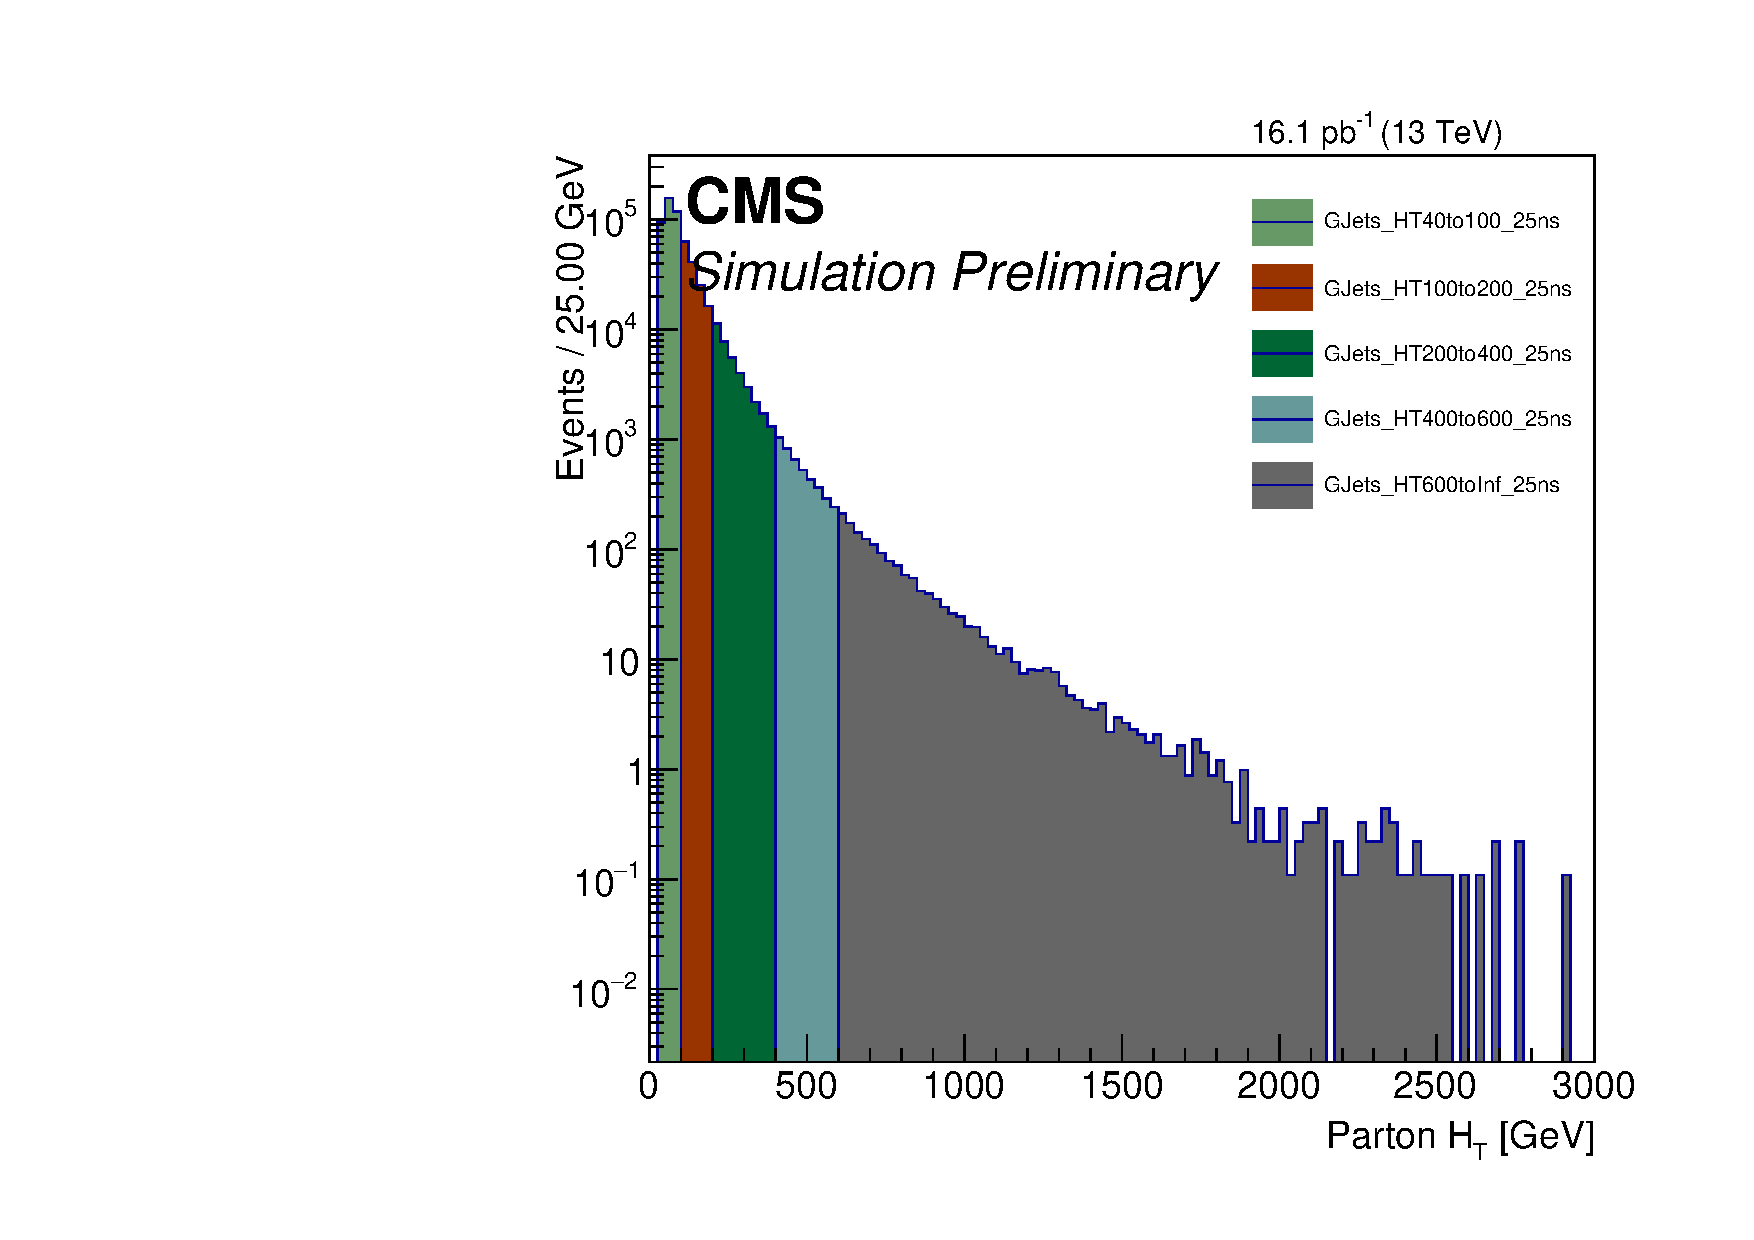
\includegraphics[width=0.45\textwidth]{figures/binnedMCsamples/GJets_HT.pdf}} ~~
    \subfigure[QCD $\hat{P_{T}}$]{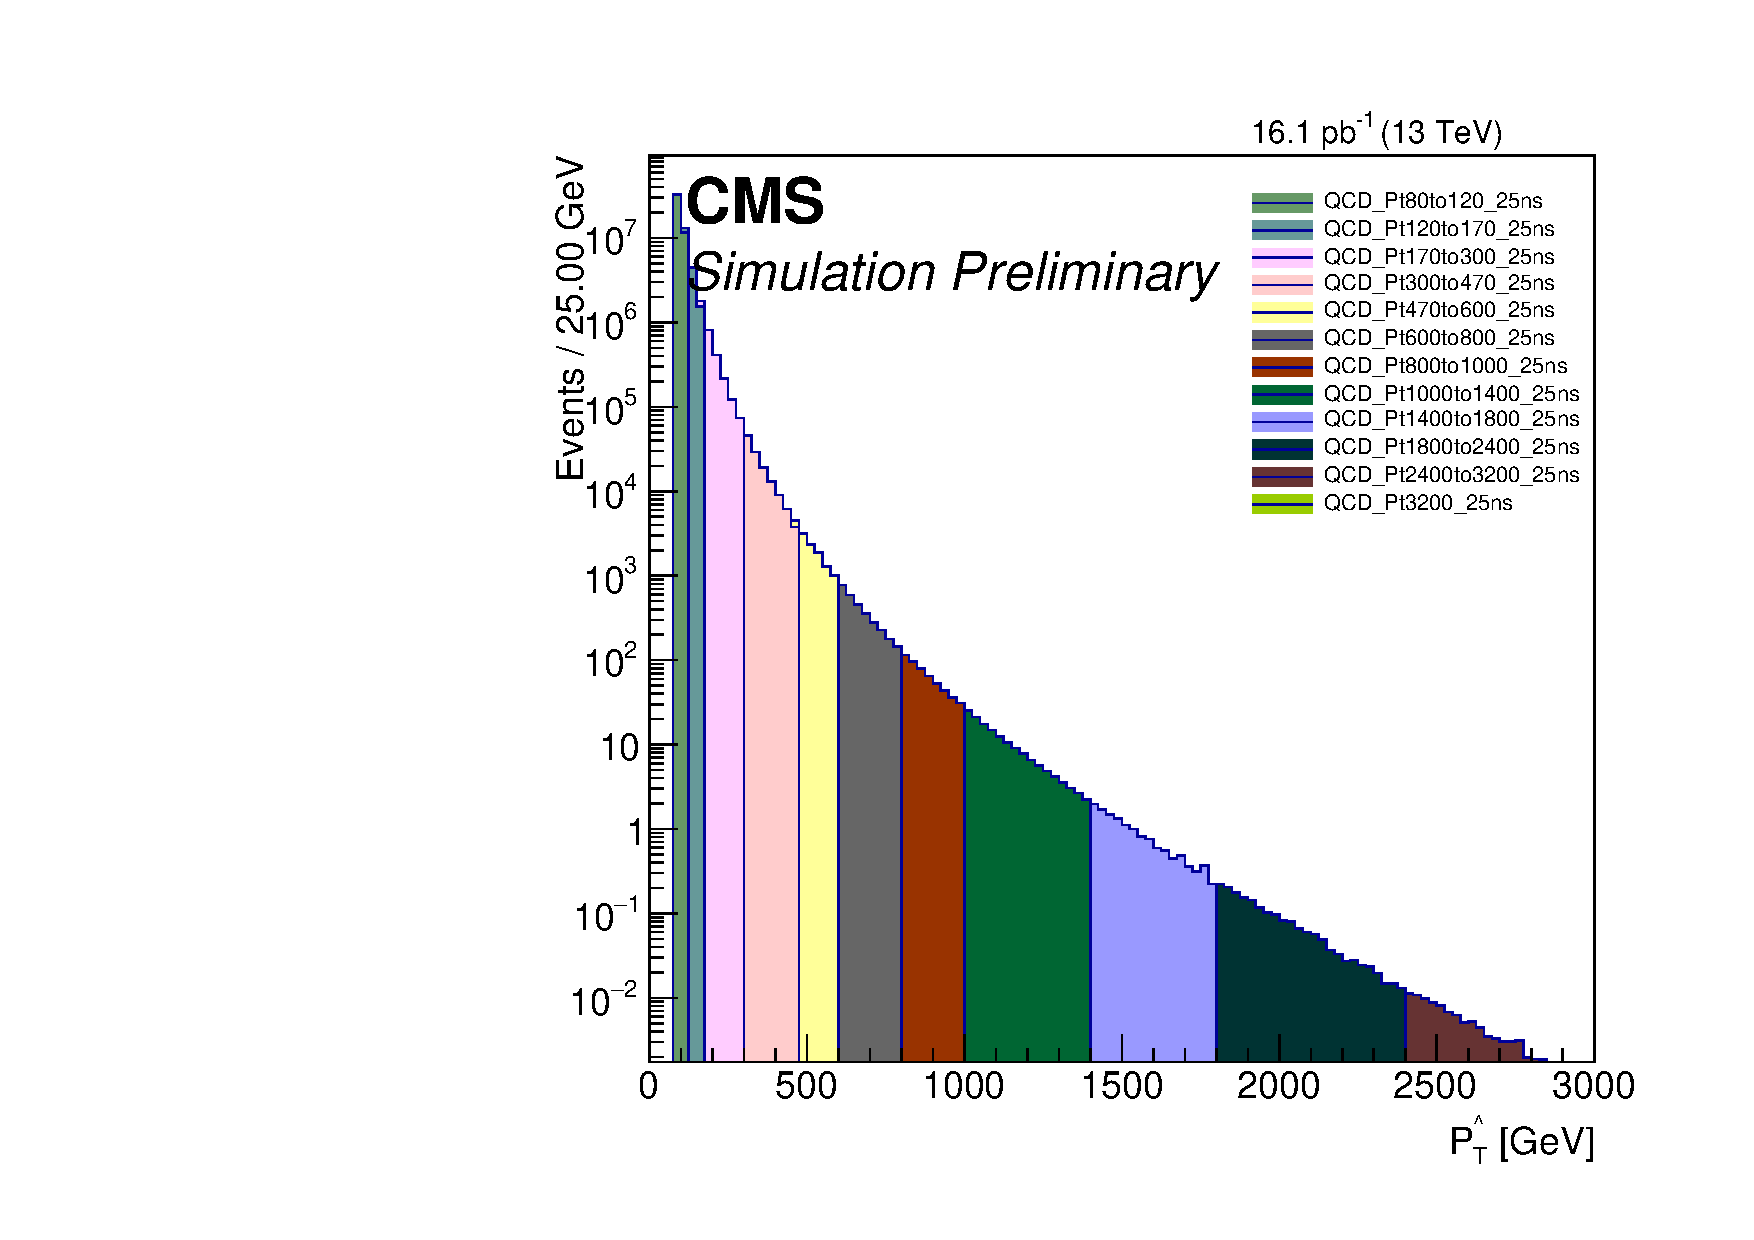
\includegraphics[width=0.45\textwidth]{figures/binnedMCsamples/QCD.pdf}}\\
    \caption{Generator-level $H_{T}^{parton}$ distributions for SM process, $Z\rightarrow \nu\nu$ + jets, W+jets, DY+jets, QCD, $\gamma$+jets, and $\hat{P_{T}}$ for QCD.}
    \label{fig:Lhe_Ht}
  \end{center}
\end{figure}

%%____________________________________________________________________________||
